\documentclass{article}

\title{Dummit \& Foote Ch. 3.2: More on Cosets and Lagrange's Theorem}
\author{Scott Donaldson}
\date{Oct. 2023}
\usepackage{amsmath, amsthm, amsfonts, enumitem, tabu, tikz}

\begin{document}

\maketitle

Let $G$ be a group.

\section*{1. (10/1/23)}

Which of the following are permissible orders of subgroups of a group of order 120: 1, 2, 5, 7, 9, 15, 60, 240? For each permissible order give the corresponding index.

\begin{proof}
    From Lagrange's theorem, the order of a subgroup of a group of order 120 must divide 120. Then the permissible orders for subgroups are $1 = \frac{120}{120}$, $2 = \frac{120}{60}, 5 = \frac{120}{24}, 15 = \frac{120}{8}$, and $60 = \frac{120}{2}$. For each of these orders the index is given by the corresponding denumerator.
\end{proof}

\section*{2. (10/2/23)}

Prove that the lattice of subgroups of $S_3$ below is correct (i.e., prove that it contains all subgroups of $S_3$ and that their pairwise joins and intersections are correctly drawn).

\begin{center}
    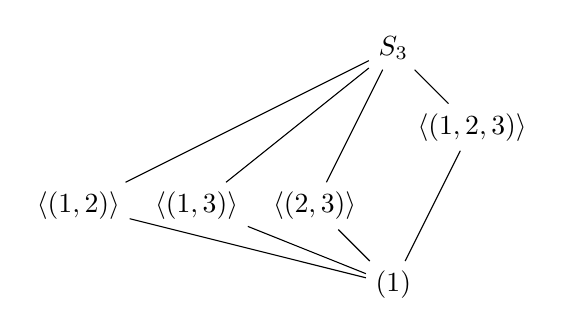
\begin{tikzpicture}
        \node at (0, 0)          (1)  {$(1)$};
        \node at (-4, 1)      (12)  {$\langle (1, 2) \rangle$};
        \node at (-2.5, 1)      (13) {$\langle (1, 3) \rangle$};
        \node at (-1, 1)      (23) {$\langle (2, 3) \rangle$};
        \node at (1, 2)      (123) {$\langle (1, 2, 3) \rangle$};
        \node at (0, 3)       (S3)  {$S_3$};
        
        \draw (1) -- (12);
        \draw (1) -- (13);
        \draw (1) -- (23);
        \draw (1) -- (123);
        \draw (12) -- (S3);
        \draw (13) -- (S3);
        \draw (23) -- (S3);
        \draw (123) -- (S3);
    \end{tikzpicture}
\end{center}

\begin{proof}
    The symmetric group $S_3$ contains 6 elements. By Lagrange's theorem, its proper subgroups must have order 2 or 3. Each of the subgroups in the lattice above have order 2 or 3, so there are no smaller or larger subgroups not depicted above.

    From Corollary 10, a subgroup of order 2 must be isomorphic to $Z_2$, that is, cyclic and generated by a single element of order 2. The three subgroups generated by the three elements of order 2 (the 2-cycles of $S_3$) are depicted above. Similarly, a subgroup of order 3 must be isomorphic to $Z_3$ and generated by a single element of order 3. The subgroup generated by $(1, 2, 3)$ contains $(1, 3, 2)$, so there is only a single subgroup of order 3.

    Next, again by Lagrange's Theorem, a subgroup of two different containing groups must have an order that divides the order of both of the containing groups. First consider a subgroup of order 2 and a subgroup of order 3. Only 1 divides 2 and 3, so the intersection must be the identity. Similarly, if a subgroup of order 2 and a subgroup of order 3 are contained in a larger group, then that group's order must have both 2 and 3 as divisors. The smallest integer for which this is possible is 6, which is the order of all of $S_3$.

    Finally, consider a pair of subgroups of order 2. Their intersection is either the identity or else they are the same subgroup. Their join must have even order, but 4 does not divide 6 and any larger even number exceeds the order of $S_3$. Thus their join is all of $S_3$. This concludes the proof that the lattice of subgroups of $S_3$ is correct.
\end{proof}

\section*{3. (10/2/23)}

Prove that the lattice of subgroups of $Q_8$ below is correct.

\begin{center}
    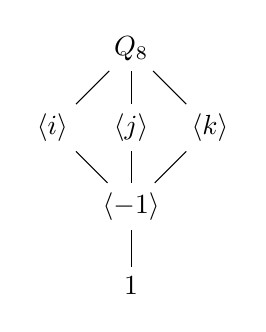
\begin{tikzpicture}
        \node at (0, 0)          (1)  {$1$};
        \node at (0, 1)      (-1)  {$\langle -1 \rangle$};
        \node at (-1, 2)      (i) {$\langle i \rangle$};
        \node at (0, 2)      (j) {$\langle j \rangle$};
        \node at (1, 2)      (k) {$\langle k \rangle$};
        \node at (0, 3)       (Q8)  {$Q_8$};
        
        \draw (1) -- (-1);
        \draw (-1) -- (i);
        \draw (-1) -- (j);
        \draw (-1) -- (k);
        \draw (i) -- (Q8);
        \draw (j) -- (Q8);
        \draw (k) -- (Q8);
    \end{tikzpicture}
\end{center}

\begin{proof}
    The group $Q_8$ has order $8 = 2^3$, so by Lagrange's theorem its proper subgroups must have order 2 or 4. We will start from the bottom and work toward the top: There is only one element of order 2 in $Q_8$, $-1$, and the cyclic subgroup generated by it is in the lattice.

    For each of $i, j$, and $k$, $\langle -1 \rangle$ is contained in the subgroup generated by them (ex. $\langle i \rangle = \{ \pm{1}, \pm{i} \}$) and there are no intermediate subgroups, since there is no divisor of 4 that is strictly greater than 2. At this point, every element of $Q_8$ is represented, so there are no cyclic subgroups missing. We might ask if there is a subgroup of order 4 missing. If so, it cannot be cyclic, and from Ch. 1.1, Exercise 36, it must be isomorphic to $V_4$. However, $V_4$ contains three elements of order 2, and $Q_8$ only has one, so there is no subgroup of $Q_8$ isomorphic to $V_4$.

    Finally, the join of any of the subgroups generated by $i, j$, or $k$ must contain strictly more than 4 elements and its order must divide 8. Then any of their joins must have order 8, that is, be all of $Q_8$.
\end{proof}

\section*{4. (10/3/23)}

Show that if $|G| = pq$ for some primes $p$ and $q$ (not necessarily distinct) then either $G$ is abelian or $Z(G) = 1$.

\begin{proof}
    We will show, equivalently, that if $|Z(G)| > 1$, then $G$ is abelian.
    
    Let $x \in Z(G)$. From Corollary 9, the order of $x$ divides $|G| = pq$. If $|x| = pq$, then $G = \langle x \rangle$ and so is abelian. Suppose without loss of generality that $|x| = p$. Now since the center of a group is a subgroup, we must have $\langle x \rangle \leq Z(G)$. If there exists a $y \in Z(G), y \notin \langle x \rangle$, then the order of $Z(G)$ exceeds $p$ and must divide $pq$, then it must be all of $G$ and hence $G$ is abelian. So suppose $Z(G) = \langle x \rangle$.
    
    The center of a group is normal in that group, so $G/Z(G)$ is well-defined. Since $|Z(G)| = p$, it has $q$ cosets in $G$; that is, the quotient group $G/Z(G)$ has prime order $q$ and is thus isomorphic to $Z_q$, hence cyclic. From Ch. 3.1, Exercise 36., $G$ is thus abelian.
\end{proof}

\section*{5. (10/4/23)}

Let $H$ be a subgroup of $G$ and fix some element $g \in G$.

\begin{enumerate}[label=(\alph*), itemsep=0em]
    \item Prove that $gHg^{-1}$ is a subgroup of $G$ of the same order as $H$.
          \begin{proof}
            By definition elements of $gHg^{-1}$ can be written in the form $ghg^{-1}$ for some $h \in H$, so let $gh_1g^{-1}, gh_2g^{-1} \in gHg^{-1}$. Then we have:
            \begin{equation*}
                (gh_1g^{-1})(gh_2g^{-1})^{-1} = gh_1g^{-1}gh_2^{-1}g_1 = gh_1h_2^{-1}g^{-1} \in gHg^{-1},
            \end{equation*}
            so $gHg^{-1}$ fulfills the subgroup criterion and is thus a subgroup of $G$.

            Next, let $\varphi_g: H \rightarrow gHg^{-1}$ be defined by $\varphi_g(h) = ghg^{-1}$ for all $h \in H$. This map is injective by the cancellation laws: $gh_1g^{-1} = gh_2g^{-1}$ implies that $h_1 = h_2$. It is also surjective: Let $x \in gHg^{-1}$. By definition $x = ghg^{-1}$ for some $h \in H$, so $\varphi_g(h) = x$. Therefore $\varphi_g$ is a bijection, and so $H$ and $gHg^{-1}$ have the same order.
          \end{proof}
    \item Deduce that if $n \in \mathbb{Z}^+$ and $H$ is the unique subgroup of $G$ of order $n$ then $H \unlhd G$.

          Suppose that $H$ is the unique subgroup of order $n$ in $G$. Then for all $g \in G$, we must have $gHg^{-1} = H$ (it cannot be any other subgroup, because $|gHg^{-1}| = |H| = n$ and there is no other subgroup of order $n$ in $G$). It follows that $H$ is normal in $G$.
\end{enumerate}

\section*{6. (10/4/23)}

Let $H \leq G$ and let $g \in G$. Prove that if the right coset of $Hg$ equals \emph{some} left coset of $H$ in $G$ then it equals the left coset $gH$ and $g$ must be in $N_G(H)$.

\begin{proof}
    Suppose $Hg = xH$ for some $x \in G$. Now $g \in Hg$, so we must also have $g \in xH$. Then $g = xh$ for some $h \in H$. It follows that $x = gh^{-1}$. So $Hg = xH = (gh^{-1})H = gH$, which in turns implies that $gHg^{-1} = H$. Therefore $g \in N_G(H)$.
\end{proof}

\section*{7. (10/5/23)}

Let $H \leq G$ and define a relation $\sim$ on $G$ by $a \sim b$ if and only if $b^{-1}a \in H$. Prove that $\sim$ is an equivalence relation and describe the equivalence class of each $a \in G$. Use this to prove Proposition 4.

\begin{proof}
    Let $a, b, c \in G$. We have $a \sim a$, because $a^{-1} a = 1 \in H$. If $a \sim b$, then we have $b^{-1}a \in H$. Now $b \sim a = a^{-1}b = (b^{-1}a)^{-1} \in H$, since $H$ is closed under inverses, so $a \sim b$ implies that $b \sim a$ (and the logic holds in reverse). Finally, if $a \sim b$ and $b \sim c$, then $b^{-1}a, c^{-1}b \in H$. Then their product, $c^{-1}bb^{-1}a = c^{-1}a$, is an element of $H$, which implies $a \sim c$. The relation $\sim$ is reflexive, symmetric, and transitive, therefore it is an equivalence relation.

    Let $a \in G$ and let $b$ lie in the left coset $aH$, so $b = ah$ for some $h \in H$. Then $b^{-1}a = (ah)^{-1}a = h^{-1}a^{-1}a = h^{-1} \in H$, so $a \sim b$. This implies that $aH$ is a subset of the equivalence class of $a$. And, if we have $a \sim b$, then $b^{-1}a \in H$, so $b^{-1}a = h$ for some $h \in H$. It follows that $b = ah^{-1} \in aH$, so the equivalence class of $a$ is a subset of $aH$. Since each is contained in the other, the equivalence class of $a$ under $\sim$ is the left coset $aH$.

    Now Proposition 4 states that:
    \begin{itemize}[itemsep=0em]
        \item The set of left cosets of $H$ in $G$ form a partition of $G$.
        \item For all $a, b \in G, aH = bH$ if and only if $b^{-1}a \in H$.
        \item In particular, $aH = bH$ if and only if $a$ and $b$ are representatives of the same coset.
    \end{itemize}
    Since the equivalence class of $a$ under $\sim$ is exactly the left coset $aH$ and equivalence classes partition a set, the left cosets of $H$ in $G$ partition $G$. The proof for the remaining items follows directly from the proof above that $a \sim b \iff b^{-1}a \in H \iff b \in aH$.
\end{proof}

\end{document}